\documentclass[Japanese]{dicomopapers}
%\documentclass[Japanese,noauthor]{dicomopapers}

\usepackage[dvips]{graphicx}
\usepackage{latexsym}

\def\Underline{\setbox0\hbox\bgroup\let\\\endUnderline}
\def\endUnderline{\vphantom{y}\egroup\smash{\underline{\box0}}\\}
\def\|{\verb|}

\begin{document}

% 和文表題
\title{IoTデバイスの通信セキュリティ向上のための\\ホームネットワーク仮想化フレームワークの提案}
% 英文表題
\etitle{Proposal of Home Network Virtualization Framework\\to Improve Communication Security of IoT Devices}

% 所属ラベルの定義
\affiliate{DOSHISHA}{同志社大学大学院 理工学研究科\\Graduate School of Science and Engineering, Doshisha University}
\affiliate{MOBILITY}{同志社大学モビリティ研究センター\\Mobility Reserch Center, Doshisha University}

\author{塚崎 拓真}{TAKUMA TSUKASAKI}{DOSHISHA}
\author{滕 睿}{RUI TENG}{MOBILITY}
\author{佐藤 健哉}{KENYA SATO}{DOSHISHA}

\begin{abstract}
  このパンフレットは,DICOMO2022に投稿する論文の最終版を,日本語
  {\LaTeX} を用いて作成し提出するためのガイドである.このパンフレットで
  は,論文作成のためのスタイルファイルについて解説している.また,このパ
  ンフレット自体も論文と同じ方法で作成されているので,必要に応じてスタイ
  ルファイルとともに配布するソース・ファイルを参照されたい.また,本スタ
  イルファイルの元になっているのは,情報処理学会論文誌用のスタイルファイ
  ル( https://www.ipsj.or.jp/journal/submit/style.html からアクセス可能)
  なので,{\LaTeX}コマンドの詳細などについては,それらを参照されたい.
  \underline{\bf なお,論文フォーマットについては,上記の原稿執筆案内に
    記載されたフォーマットではなく,本フォー}\\
  \underline{\bf マットをご利用いただきたい.}

\end{abstract}

% 表題などの出力
\maketitle

% 本文はここから始まる
\section{はじめに}
近年,IoT(Internet of Things)が注目を集めるようになり,今後あらゆるモノがネットワークに接続され,利用されることが予想される.\par
しかし,IoTの発展により利便性が高まる一方で,これまでネットワークに接続されていなかったモノが接続されることにより,セキュリティ上のリスクも高まっている.
IoTデバイスは十分なセキュリティを考慮せずに開発されたものが多いため,悪意のある攻撃者によるサイバー攻撃の標的になりやすい.
また,現在のスマートホームデバイスは,クラウド上のシステムと連携することで,デバイス間の連携を可能にしているが,今後はホームネットワーク内で閉じたデバイス間の通信によって連携を行う形になることが想定される.
デバイス間で直接通信を行う場合,各デバイスにおいてどのデバイスとの通信を受け入れるか,アクセス制御を行う必要がある.
% セキュリティ上の脅威が各種デバイスに顕在した場合,個別に対処するとコストや時間がかかってしまうため,脅威に対し一括に対処する必要がある.\par
% しかし,ホームネットワーク内には異なる規格のハードウェアや様々なアプリケーションが混在しているため,それら全てに対応したシステムの構築や更新を続けるのは困難である.
% しかし,全てのデバイスがアクセス制御に対応しているとは限らず,デバイスの計算能力の制限によって実現できるアクセス制御に制限がある場合や,デバイスのソフトウェア自体の脆弱性によってアクセス制御が機能しない場合が考えられる.
しかし,IoTデバイスは従来のPC等の既存機器と比較した場合,CPU等のリソースを十分に保持していないため,デバイスの計算能力の制限やソフトウェア自体の脆弱性によって,適用できる機能が限られるという問題がある.
そのため,ホームネットワーク内で通信するのであれば,どのデバイスも必ず利用するネットワークを利用したシステムを構築することが望ましい.\par
そこで本研究では,SDN(Software Defined Networks)の代表的プロトコルであるOpenFlowを用いて,ホームネットワーク内の通信を監視するフレームワークの構築を検討した.
% OpenFlowを利用することで,既存IoTデバイスや異なる規格などに対応でき,ホームネットワークに適した形で不正な通信の検知を実現する.
提案システムでは,セキュリティ対策を適用可能なデバイスをProxyと定義し,ルータ上に仮想的に作成する.
ここに,IoTデバイスがリソース量の制限により適用できないセキュリティ対策をオフロードし,このProxyがIoTデバイス間の通信を中継することで,本来IoTデバイスに適用したいセキュリティ対策を実現する.
セキュリティ対策として,ホームネットワーク内の通信のトラフィック情報は既知であることを考慮し,フローの検証をOpenFlowコントローラで行う.\par
ルータ内にコンテナを配置し,そのコンテナ上にProxyを作成する.そして,IoTデバイス間で閉じた通信を行うシミュレーションの評価を行い,ホームネットワークにおいてセキュリティ要件を保つことを示した.

\begin{figure}[!tb]
  \centering
  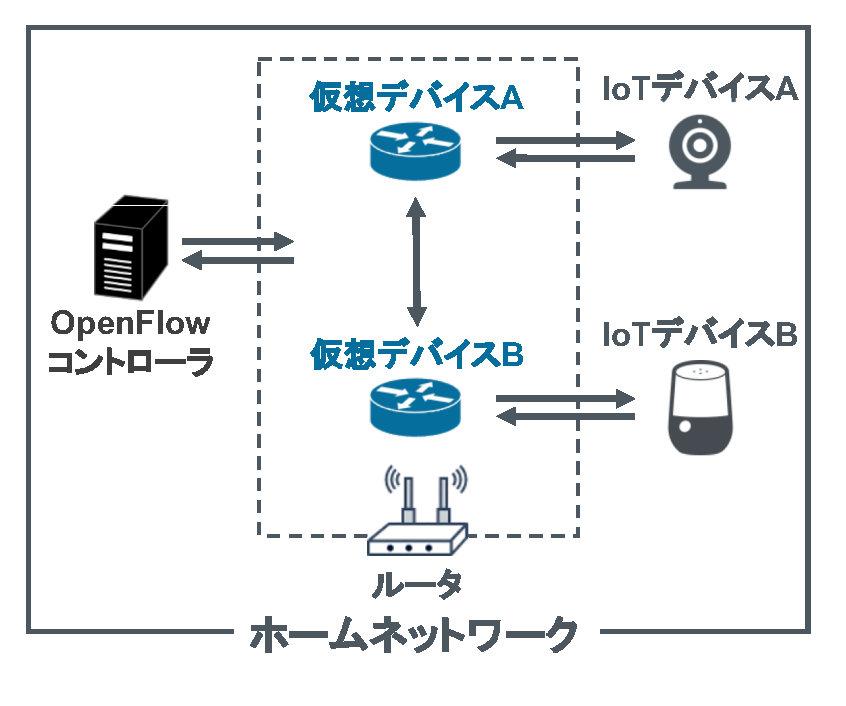
\includegraphics[width=\linewidth]{img/system.eps}
  \caption{提案システムの構成}
  \label{fig:system}
\end{figure}

\section{関連研究}

\section{提案システム}

\section{実装}

\section{結果と考察}

\section{まとめ}

\begin{thebibliography}{10}
  \bibitem{webpage}
  情報処理学会: 情報処理学会論文誌(IPSJ Journal)原稿執筆案内,情報処理学
  会(オンライン),
  \urlj{https://\\www.ipsj.or.jp/journal/submit/ronbun\_j\_prms.html}
  \refdatej{2022-03-01}.
\end{thebibliography}

\end{document}
